% Created 2015-06-21 Dom 18:40
\documentclass[11pt]{article}
\usepackage[utf8]{inputenc}
\usepackage[T1]{fontenc}
\usepackage{fixltx2e}
\usepackage{graphicx}
\usepackage{longtable}
\usepackage{float}
\usepackage{wrapfig}
\usepackage{rotating}
\usepackage[normalem]{ulem}
\usepackage{amsmath}
\usepackage{textcomp}
\usepackage{marvosym}
\usepackage{wasysym}
\usepackage{amssymb}
\usepackage{hyperref}
\tolerance=1000
\usepackage{minted}
\usemintedstyle{perldoc}
\usepackage{tikz}
\usetikzlibrary{decorations.markings}
\tikzstyle{vertex}=[circle, draw, inner sep=0pt, minimum size=7pt]
\providecommand{\vertex}{\node[vertex]}
\author{Alice Duarte Scarpa, Bruno Lucian Costa}
\date{2015-06-23}
\title{Exercício 7.28 (Tardos)}
\hypersetup{
  pdfkeywords={},
  pdfsubject={},
  pdfcreator={Emacs 24.4.1 (Org mode 8.2.10)}}
\begin{document}

\maketitle

\section{Enunciado}
\label{sec-1}

Um grupo de estudantes está escrevendo um módulo para preparar
cronogramas de monitoria. O protótipo inicial deles funciona do
seguinte modo: O cronograma é semanal, de modo que podemos nos focar
em uma única semana.

\begin{itemize}
\item O administrador do curso escolhe um conjunto de $k$
intervalos disjuntos de uma hora de duração $I_1, I_2, \ldots,
      I_k$, nos quais seria possível que monitores dessem suas
monitorias; o cronograma final consistirá de um subconjunto de
alguns (mas geralmente não todos) esses intervalos.
\item Cada monitor então entra com seu horário semanal, informando
as horas em que ele está disponível para monitorias.
\item O administrador então especifica, para parâmetros $a$, $b$ e
$c$, que cada monitor deve dar entre $a$ e $b$ horas de
monitoria por semana, e que um total de $c$ horas de monitoria
deve ser dado semanalmente.
\end{itemize}

O problema é escolher um subconjunto dos horários (intervalos) e
atribuir um monitor a cada um desses horários, respeitando a
disponibilidade dos monitores e as restrições impostas pelo
administrador.


a) Dê um algoritmo polinomial que ou constrói um cronograma
   válido de horas de monitoria (especificando que monitor cobre
   quais horários) ou informa que não há cronograma válido.


b) O algoritmo acima tornou-se popular, e surgiu a vontade de
   controlar também a densidade das monitorias: dado números $d_i$,
   com $i$ entre $1$ e $5$, queremos um cronograma com pelo menos
   $d_i$ horários de monitoria no dia da semana $i$. Dê um
   algoritmo polinomial para resolver o problema com essa restrição
   adicional.


\section{Introdução}
\label{sec-2}

Queremos modelar esse problema como um problema de fluxo. Para isso
vamos começar com algumas definições de fluxo.

\subsection{Definições}
\label{sec-2-1}

Uma rede de fluxo é um grafo direcionado $G =
(V, E)$ com as seguintes propriedades:
\begin{itemize}
\item Existe um único vértice \textit{fonte} $s \in V$. Nenhuma aresta entra em $s$.
\item A cada aresta $e$ está associada uma capacidade inteira $c_e$ e
uma demanda $d_e$ tal que $c_e \geq d_e \geq 0$.
\item Existe um único vértice \textit{dreno} $t \in V$. Nenhuma aresta sai de $t$.
\end{itemize}

Um fluxo $f$ de $s$ a $t$ é uma função $f \colon E \to R^+$ que associa a cada
aresta $e$ um valor real não-negativo $f(e)$ tal que:

\begin{enumerate}
\item $\forall e \in E, d_e \leq f(e) \leq c_e$
\item Para todo nó $v \not\in \{s,t\}$:
\[ \sum_{e \text{ chegando em } v} f(e) = \sum_{e \text{ saindo de } v} f(e) \]
\end{enumerate}

$f(e)$ representa o fluxo que vai passar pela aresta $e$. O valor de
um fluxo é o total que parte da fonte $s$, isso é:

\begin{equation}
\label{valor_fluxo} \mathrm{Valor}(f) = \sum_{e \text{ saindo de } s} f(e)
\end{equation}

\subsection{Representação}
\label{sec-2-2}

Vamos usar uma classe para representar arestas. Uma aresta é
inicializada com as propriedades: vértice de origem, vértice de
destino, capacidade e demanda.

Para facilitar o processamento futuro, vamos adicionar também as
propriedades reversa e original. Reversa aponta para uma outra aresta
reversa à atual, a propriedade original é uma flag indicando se a
aresta pertence à rede original ou não.
\begin{minted}[]{python}
class Aresta():
    def __init__(self, origem, destino, capacidade, demanda):
        self.origem = origem
        self.destino = destino
        self.capacidade = capacidade
        self.demanda = demanda
        self.reversa = None
        self.original = True
\end{minted}

Agora que temos a classe Aresta, vamos usá-la para auxiliar na
representação de uma rede de fluxo também como objeto.

Uma rede de fluxo tem duas propriedades: adjacências, um dicionário
que mapeia cada vértice às arestas que saem dele e fluxo.

O construtor da classe inicializa as duas propriedades como dicionários vazios.

Vamos precisar dos seguintes métodos na nossa classe RedeDeFluxo:

\begin{itemize}
\item \verb~novo_vertice(v)~: Adiciona o vértice v à rede
\item \verb~nova_aresta(origem, destino, capacidade)~: Adiciona uma nova aresta a
rede. Também cria a aresta reversa.
\item \verb~novo_fluxo(f, e)~: Adiciona um fluxo $f$ à aresta $e$
\item \verb~encontra_arestas(v)~: Retorna as arestas que partem do vértice $v$
\item \verb~valor_do_fluxo(fonte)~: Encontra o valor do fluxo, como definido em \eqref{valor_fluxo}.
\end{itemize}

\begin{minted}[]{python}
class RedeDeFluxo():
    def __init__(self):
        self.adj = collections.OrderedDict()
        self.fluxo = {}

    def novo_vertice(self, v):
        self.adj[v] = []

    def nova_aresta(self, origem, destino, capacidade, demanda):
        aresta = Aresta(origem, destino, capacidade, demanda)
        self.adj[origem].append(aresta)

        # Criando a aresta reversa
        aresta_reversa = Aresta(destino, origem, 0, -demanda)
        self.adj[destino].append(aresta_reversa)
        aresta_reversa.original = False

        # Marcando aresta e aresta_reversa como reversas uma da outra
        aresta.reversa = aresta_reversa
        aresta_reversa.reversa = aresta

    def novo_fluxo(self, e, f):
        self.fluxo[e] = f

    def encontra_arestas(self, v):
        return self.adj[v]

    def valor_do_fluxo(self, fonte):
        valor = 0
        for aresta in self.encontra_arestas(fonte):
            valor += self.fluxo[aresta]
        return valor
\end{minted}

\section{Modelando o problema com fluxos\label{modelagem_fluxo}}
\label{sec-3}

Os dois itens do problema podem ser reduzidos a encontrar um fluxo
válido em uma rede usando construções semelhantes.

Para o item a), construimos o grafo da seguinte forma:

\begin{itemize}
\item Criamos um vértice $s$ representando a fonte e um vértice $t$
  representando o dreno
\item Para cada intervalo $I_i \in I_1, I_2, \ldots, I_k$ escolhido pelo
administrador, criamos um vértice $I_i$ e uma aresta $(s, I_i)$
capacidade 1 e demanda 0
\item Para cada monitor $T_i \in T_1, T_2, \ldots, T_m$ criamos um vértice
$T_i$. Se o monitor está disponível para dar monitoria no intervalo
$I_j$ criamos uma aresta de $(I_j, T_i)$ de demanda 0 e
capacidade 1. Para cada monitor também criamos uma aresta
$(T_i, t)$ de demanda $a$ e capacidade $b$.
\item Para garantir que a solução final terá exatamente $c$ horas de
monitoria, criamos uma nova fonte $s'$ e uma aresta $(s', s)$
com demanda e capacidade $c$.
\end{itemize}

Para construir uma atribuição de intervalos válida a partir de um
fluxo, é suficiente atribuir um intervalo a um monitor se a aresta que
liga o intervalo ao monitor tem fluxo 1.  As condições de capacidade e
demanda da rede garantem que um intervalo é atribuído a no máximo um
monitor, que cada monitor recebe apenas intervalos compatíveis com ele
e que as restrições no número de hora são satisfeitas.

Reciprocamente, para toda atribuição de intervalos válida, podemos
construir um fluxo passando uma unidade de fluxo pelo caminho $(s', s, I,
T, t)$ para cada par $(I, T)$ de intervalo e monitor correspondente. A
validade da atribuição implica imediatamente que as condições de
demanda e capacidade são atendidas.

O caso com 3 intervalos e 2 monitores (A e B) em que o monitor A está
disponível nos intervalos 1 e 2 e o monitor B está disponível nos
horários 1 e 3 está representado abaixo. Os rótulos
das arestas são da forma demanda/capacidade. As
arestas sem rótulo tem demanda 0 e capacidade 1.


\[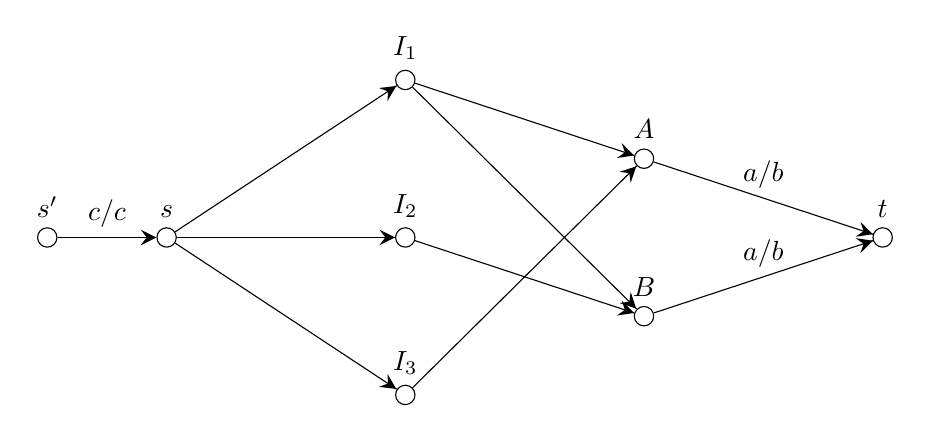
\begin{tikzpicture}[x=0.25\textwidth,
    every edge/.style={
        draw,
        postaction={decorate,
                    decoration={markings,mark=at position 1 with {\arrow[line width = 0.5mm]{stealth}}}
                   }
        }
]
\vertex (fonte') at (0,3) [label=above:$s$] {};
\vertex (fonte) at (-0.5,3) [label=above:$s'$] {};
\vertex (I1) at (1,5) [label=above:$I_1$] {};
\vertex (I2) at (1,3) [label=above:$I_2$] {};
\vertex (I3) at (1,1) [label=above:$I_3$] {};
\vertex (A) at (2,4) [label=above:$A$] {};
\vertex (B) at (2,2) [label=above:$B$] {};
\vertex (dreno) at (3,3) [label=above:$t$] {};
\path
(fonte) edge node [above] {$c/c$} (fonte')
(fonte') edge (I1)
(fonte') edge (I2)
(fonte') edge (I3)
(I1) edge (A)
(I1) edge (B)
(I2) edge (B)
(I3) edge (A)
(A) edge node [above] {$a/b$} (dreno)
(B) edge node [above] {$a/b$} (dreno)
;
\end{tikzpicture}\]

A única diferença na construção do item b é que, ao invés de ligarmos
$s$ diretamente aos intervalos de monitoria, ligamos $s$ a cada dia da
semana i com demanda $d_i$ e capacidade $c$ e depois
criamos uma aresta com demanda 0 e capacidade 1 de
cada dia da semana para os intervalos que são naquele dia.

Abaixo está o mesmo exemplo do item a) com dias da semana. Para deixar
a visualização mais simples estamos colocando aqui apenas dois dias da
semana.

\[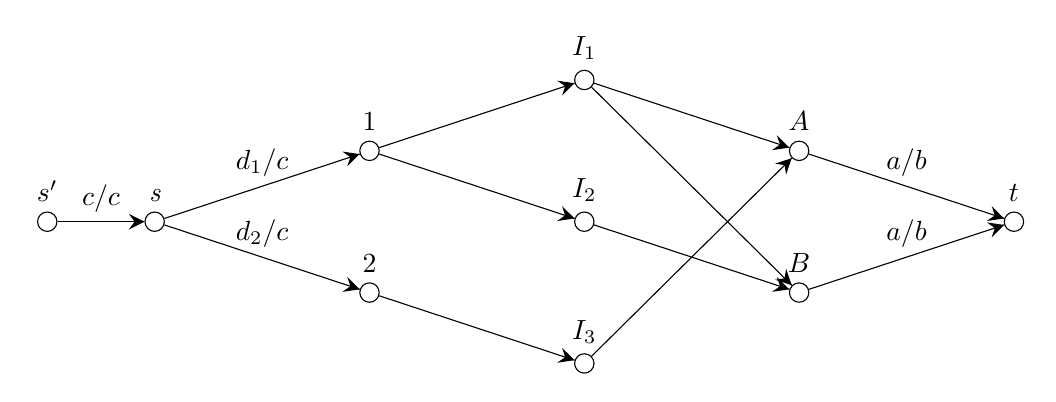
\begin{tikzpicture}[x=0.25\textwidth, scale=0.9,
    every edge/.style={
        draw,
        postaction={decorate,
                    decoration={markings,mark=at position 1 with {\arrow[line width = 0.5mm]{stealth}}}
                   }
        }
]
\vertex (fonte') at (0,3) [label=above:$\textit{s}$] {};
\vertex (fonte) at (-0.5,3) [label=above:$s'$] {};
\vertex (1) at (1, 4) [label=above:$1$] {};
\vertex (2) at (1, 2) [label=above:$2$] {};
\vertex (I1) at (2,5) [label=above:$I_1$] {};
\vertex (I2) at (2,3) [label=above:$I_2$] {};
\vertex (I3) at (2,1) [label=above:$I_3$] {};
\vertex (A) at (3,4) [label=above:$A$] {};
\vertex (B) at (3,2) [label=above:$B$] {};
\vertex (dreno) at (4,3) [label=above:$t$] {};
\path
(fonte) edge node [above] {$c/c$} (fonte')
(fonte') edge node [above] {$d_1/c$} (1)
(fonte') edge node [above] {$d_2/c$} (2)
(1) edge (I1)
(1) edge (I2)
(2) edge (I3)
(I1) edge (A)
(I1) edge (B)
(I2) edge (B)
(I3) edge (A)
(A) edge node [above] {$a/b$} (dreno)
(B) edge node [above] {$a/b$} (dreno)
;
\end{tikzpicture}\]

\section{Implementação}
\label{sec-4}

\subsection{Fluxo máximo}
\label{sec-4-1}

Vamos começar estudando o problema de encontrar o fluxo máximo de uma
rede $G$ em que $d_e = 0 \; \forall e \in E$ $f$. Vamos implementar aqui o
algoritmo de Ford-Fulkerson para resolver esse problema.

O algoritmo tem 2 partes:

\begin{enumerate}
\item Dado um caminho $P$ e partindo de um fluxo inicial $f$, obter um
novo fluxo $f'$ expandindo $f$ em $P$
\item Partindo do fluxo $f(e)$ = 0, expandir o fluxo enquanto for possível
\end{enumerate}


\begin{itemize}
\item Primeira parte:
\end{itemize}

Queremos expandir o fluxo $f$ em $P$. Mais precisamente, queremos
mudar o valor do fluxo somando $x$ ao valor de $f(e)$ para toda aresta
$e$ que está no caminho $P$.

O gargalo de um caminho $P$ (com relação a um fluxo $f$) é o maior
valor de $x$ tal que $f(e) + x \leq c_e$ para toda aresta $e \in
P$. Essa última condição significa que o fluxo

\[ f'(e) = \begin{cases}f(e)&\text{ se } e \not\in P \\
                        f(e) + x&\text{ se } e \in P\end{cases} \]

ainda satisfaz as restrições de capacidade. O código abaixo computa
tal valor de $x$.
\begin{minted}[]{python}
def encontra_gargalo(self, caminho):
    residuos = []
    for aresta in caminho:
        residuos.append(aresta.capacidade - self.fluxo[aresta])
    return min(residuos)
\end{minted}

Como descrito acima, expandir o caminho é somar $x$ ao valor de $f(e)$
para cada aresta do caminho. Precisamos atualizar também as arestas
reversas, pois elas precisam satisfazer a propriedade $f(e) =
-f(e.reversa)$.
\begin{minted}[]{python}
def expande_caminho(self, caminho):
    gargalo = self.encontra_gargalo(caminho)
    for aresta in caminho:
        self.fluxo[aresta] += gargalo
        self.fluxo[aresta.reversa] -= gargalo
\end{minted}

Pela definição de gargalo, a operação de expandir $P$ gera um fluxo
válido. Se garantirmos que $c_e - f(e)$ é positivo para toda $e \in
P$, então o gargalo também será positivo, de modo que o fluxo $f'$
obtido terá valor maior que o anterior.

Tendo a restrição acima em mente, iremos fazer uma DFS no grafo,
usando apenas as arestas que possuem $c_e - f(e)$ (chamaremos esse
valor de \verb~residuo~) positivo.

Mais precisamente, a função abaixo recebe um caminho parcialmente
construído da fonte até \verb~v~ na variável \verb~caminho~ e recursivamente
encontra uma maneira de chegar em dreno a partir de \verb~v~ usando apenas
vértices não explorados. Se um caminho de \verb~v~ a dreno não existir, a
função não retorna um valor (isto é, retorna \verb~None~).

\begin{minted}[]{python}
def encontra_caminho(self, v, dreno, caminho, visitados):
    if v == dreno:
        return caminho

    visitados.add(v)

    for aresta in self.encontra_arestas(v):
        residuo = aresta.capacidade - self.fluxo[aresta]
        if residuo > 0 and aresta.destino not in visitados:
            resp = self.encontra_caminho(aresta.destino,
                                         dreno,
                                         caminho + [aresta],
                                         visitados)
            if resp != None:
                return resp
\end{minted}

Como só chamamos a função com primeiro parâmetro igual a \verb~w~ quando
\verb~w~ não está no conjunto de vértices visitados e \verb~w~ é imediatamente
colocado em tal conjunto depois da chamada, chamamos a função uma
única vez por vértice. Como a função demora tempo proporcional ao
número de arestas que saem do vértice em questão, o tempo total gasto
em todas as chamadas da função é $O(|V| + |E|)$.

Para as outras funções, note que um caminho tem no máximo $|V|$
vértices, e portanto as funções \verb~encontra_gargalo~ e \verb~expande_caminho~
têm complexidade $O(|V|)$.

Para a parte 2, vamos precisar criar um fluxo $f$ com $f(e) = 0$ para
toda aresta $e$. Podemos fazer isso utilizando o seguinte método na
classe RedeDeFluxo():
\begin{minted}[]{python}
def cria_fluxo_inicial(self):
    for vertice, arestas in self.adj.iteritems():
        for aresta in arestas:
            self.fluxo[aresta] = 0
\end{minted}

Com todas as funções auxiliares prontas, podemos finalmente definir a
função que encontra o fluxo máximo, repetidamente aumentando o fluxo
como descrito na parte 1:
\begin{minted}[]{python}
def fluxo_maximo(self, fonte, dreno):
    self.cria_fluxo_inicial()

    caminho = self.encontra_caminho(fonte, dreno, [], set())
    while caminho is not None:
        self.expande_caminho(caminho)
        caminho = self.encontra_caminho(fonte, dreno, [], set())
    return self.valor_do_fluxo(fonte)
\end{minted}

Como o fluxo aumenta em pelo menos uma unidade por iteração e o custo
de uma iteração é $O(|V| + |E|)$, a complexidade total do algoritmo é
$O((|V|+|E|)F)$, onde $F$ é o fluxo máximo possível na rede. No caso
do exercício, $F$ é no máximo o número de intervalos e portanto
polinomial no tamanho da entrada.

\subsection{Fluxo válido com demandas não-nulas}
\label{sec-4-2}

O nosso objetivo é encontrar um fluxo válido $f$ para uma rede $G =
(V, E)$ no caso em que as demandas são positivas.

Vamos construir uma rede $G' = (V', E')$ com um valor associado $d$
tal que $d_e = 0 \; \forall e \in E'$ de tal forma que um fluxo válido
para $G$ existe se e somente se o valor do fluxo máximo em $G'$ é
$d$. Em caso afirmativo, podemos construir um fluxo válido $f$ para
$G$ rapidamente a partir de qualquer fluxo máximo $f'$ de $G'$.

Construimos $G'$ da seguinte forma:

\begin{itemize}
\item Criamos um vértice em $G'$ para cada vértice $G$
\item Adicionamos uma fonte adicional $F$ e um dreno adicional $D$ a $G'$
\item Definimos o saldo de cada vértice $v \in V$ como: \[
  \textrm{saldo}(v) = \sum_{e \text{ saindo de }v}d_e - \sum_{e \text{
  chegando em }v}d_e \]
\item Se $\mathrm{saldo}(v) > 0$ adicionamos uma aresta $(v, D,
  \mathrm{saldo}(v), 0)$ a $G'$
\item Se $\mathrm{saldo}(v) < 0$ adicionamos uma aresta $(F, v,
  -\mathrm{saldo}(v), 0)$ a $G'$
\item Para cada aresta $e = (\mathrm{origem, destino, capacidade,
  demanda}) \in E$, crie uma aresta $e' = (\mathrm{origem, destino,
  capacidade - demanda, 0})$ em $G'$
\end{itemize}

Codificando a construção acima:
\begin{minted}[]{python}
def cria_rede_com_demandas_nulas(G):
    G_ = RedeDeFluxo()
    G_.novo_vertice('F')
    G_.novo_vertice('D')
    d = 0

    for vertice, arestas in G.adj.iteritems():
        G_.novo_vertice(vertice)
        saldo = sum(e.demanda for e in arestas)
        if saldo > 0:
            G_.nova_aresta(vertice, 'D', saldo, 0)
            d += saldo
        elif saldo < 0:
            G_.nova_aresta('F', vertice, -saldo, 0)

    for arestas in G.adj.values():
        for a in arestas:
             if a.original:
                 G_.nova_aresta(a.origem,
                                a.destino,
                                a.capacidade - a.demanda,
                                0)
    return G_, d
\end{minted}

\section{Rodando o algoritmo}
\label{sec-5}

\subsection{Item A}
\label{sec-5-1}
A seguinte tabela mostra a disponibilidade dos monitores nos horários
escolhidos pelo administrador:

\begin{center}
\begin{tabular}{lccccccccc}
 & Ana & Bia & Caio & Davi & Edu & Felipe & Gabi & Hugo & Isa\\
Seg 10h &  &  &  & x &  &  &  &  & \\
Seg 14h &  &  &  &  &  & x & x & x & x\\
Seg 21h & x &  &  & x &  &  &  &  & \\
Ter 10h & x & x &  & x &  &  &  &  & \\
Ter 16h &  &  & x &  &  &  &  &  & \\
Ter 20h &  &  &  &  &  &  & x &  & x\\
Qua 9h &  &  &  &  &  & x &  &  & \\
Qua 17h &  &  & x &  &  &  &  &  & \\
Qua 19h &  &  &  &  &  &  &  & x & \\
Qui 7h &  & x &  &  &  & x &  &  & \\
Qui 13h &  &  &  &  &  &  & x &  & \\
Qui 19h &  & x &  &  & x &  &  & x & \\
Sex 7h &  &  & x &  & x &  &  &  & \\
Sex 11h & x &  &  &  & x &  &  &  & x\\
Sex 21h &  &  & x &  &  & x &  &  & x\\
\end{tabular}
\end{center}
As outras regras para monitoria estão na tabela abaixo:

\begin{center}
\begin{tabular}{lr}
Min de horas por monitor & 1\\
Max de horas por monitor & 3\\
Horas de monitoria & 10\\
\end{tabular}
\end{center}

Podemos carregar as informações das tabelas para criar uma rede como
descrita no final da Seção \ref{modelagem_fluxo}.
\begin{minted}[]{python}
# Lendo a tabela de disponibilidade
intervalos = collections.OrderedDict()
monitores = horarios[0][1:]

for disponibilidade in horarios[1:]:
    intervalos[disponibilidade[0]] = []
    for i, slot in enumerate(disponibilidade[1:]):
        if slot != '':
            intervalos[disponibilidade[0]].append(monitores[i])
\end{minted}

Lendo a tabela de regras
\begin{minted}[]{python}
min_horas = regras[0][1]
max_horas = regras[1][1]
total_horas = regras[2][1]
\end{minted}

Criando uma rede para o problema com os dados fornecidos

\begin{minted}[]{python}
def cria_rede(intervalos, monitores, min_horas, max_horas, total_horas):
    G = RedeDeFluxo()
    G.novo_vertice('Fonte')
    G.novo_vertice('Dreno')
    G.nova_aresta('Dreno', 'Fonte', total_horas, total_horas)

    # Criando um vertice para cada monitor e ligando esse vertice
    # ao dreno
    for monitor in monitores:
        G.novo_vertice(monitor)
        G.nova_aresta(monitor, 'Dreno', max_horas, min_horas)

    for intervalo, monitores_disponiveis in intervalos.iteritems():
        # Criando um vertice para cada intervalo e conectando a
        # fonte a cada um dos intervalos
        G.novo_vertice(intervalo)
        G.nova_aresta('Fonte', intervalo, 1, 0)

        # Conectando o intervalo a cada monitor disponivel nele
        for monitor in monitores_disponiveis:
            G.nova_aresta(intervalo, monitor, 1, 0)

    return G
\end{minted}

Agora é só rodar o algoritmo com o grafo obtido:
\begin{minted}[]{python}
G = cria_rede(intervalos, monitores, min_horas, max_horas, total_horas)
G_, d = cria_rede_com_demandas_nulas(G)
fluxo = G_.fluxo_maximo('F', 'D')
if fluxo == d:
    tabela_de_monitores = []
    for horario in intervalos:
        for w in G_.adj[horario]:
            if G_.fluxo[w] == 1:
                tabela_de_monitores.append([w.origem, w.destino])
    return tabela_de_monitores
else:
    return 'Impossivel'
\end{minted}

No final, obtemos ou 'Impossível' se não existir um horário compatível
ou uma tabela com um horário que atende a todas as restrições.

Para a tabela acima:
\begin{center}
\begin{tabular}{ll}
Seg 10h & Davi\\
Seg 14h & Gabi\\
Seg 21h & Ana\\
Ter 10h & Bia\\
Ter 16h & Caio\\
Ter 20h & Isa\\
Qua 9h & Felipe\\
Qua 17h & Caio\\
Qua 19h & Hugo\\
Qui 19h & Edu\\
\end{tabular}
\end{center}

\subsection{Item b}
\label{sec-5-2}

No item b, além de todas as restrições do item a, há também a
restrição de mínimo de horas por dia da semana.

Vamos expressar a nova restrição com uma tabela:

\begin{center}
\begin{tabular}{lr}
Seg & 1\\
Ter & 1\\
Qua & 2\\
Qui & 1\\
Sex & 1\\
\end{tabular}
\end{center}

Parsear a nova tabela é simples:
\begin{minted}[]{python}
minimo_por_dia = {}
for dia in min_por_dia:
    minimo_por_dia[dia[0]] = dia[1]
\end{minted}

A única função que precisamos alterar do item a é a função
\verb~cria_rede~, que agora tem que lidar com a construção mencionada na
Seção \ref{modelagem_fluxo}.

\begin{minted}[]{python}
def cria_rede(intervalos, monitores, min_horas,
              max_horas, total_horas, minimo_por_dia):
    G = RedeDeFluxo()
    G.novo_vertice('Fonte')
    G.novo_vertice('Dreno')
    G.nova_aresta('Dreno', 'Fonte', total_horas, total_horas)

    # Criando um vertice para cada monitor e ligando esse vertice
    # ao dreno
    for monitor in monitores:
        G.novo_vertice(monitor)
        G.nova_aresta(monitor, 'Dreno', max_horas, min_horas)

    # Criando um vertice para cada dia e uma aresta da Fonte
    # ao dia com demanda igual ao minimo de horas de monitoria
    # para aquele dia e capacidade suficientemente grande
    # (vamos usar o total de horas)
    dias = minimo_por_dia.keys()
    for dia in dias:
        G.novo_vertice(dia)
        G.nova_aresta('Fonte', dia, total_horas, minimo_por_dia[dia])

    for intervalo, monitores_disponiveis in intervalos.iteritems():
        # Encontrando o dia do intervalo
        for dia in dias:
            if intervalo.startswith(dia):
                dia_do_intervalo = dia

        # Criando um vertice para cada intervalo e conectando o
        # dia do intervalo a cada um dos intervalos
        G.novo_vertice(intervalo)
        G.nova_aresta(dia_do_intervalo, intervalo, 1, 0)

        # Conectando o intervalo a cada monitor disponivel nele
        for monitor in monitores_disponiveis:
            G.nova_aresta(intervalo, monitor, 1, 0)

    return G
\end{minted}

\begin{center}
\begin{tabular}{ll}
Seg 10h & Davi\\
Seg 14h & Isa\\
Seg 21h & Ana\\
Ter 10h & Bia\\
Ter 16h & Caio\\
Qua 9h & Felipe\\
Qua 17h & Caio\\
Qua 19h & Hugo\\
Qui 13h & Gabi\\
Sex 7h & Edu\\
\end{tabular}
\end{center}
% Emacs 24.4.1 (Org mode 8.2.10)
\end{document}
